\documentclass[12pt]{extarticle}
\usepackage[left = 2cm, right = 2cm, top = 2cm, bottom = 2cm]{geometry}
\usepackage{graphicx}
\usepackage{amsmath}
\usepackage{amssymb}
\usepackage{hyperref}
\usepackage{listings}

\begin{document}

\begin{flushleft}
\begin{LARGE}
\textbf{2.1}
\end{LARGE}  
\end{flushleft}

\vfill
\begin{center}
\begin{Huge}The Diffusion Equation\end{Huge}
\end{center}
\vfill

\pagebreak

\begin{center}
\textbf{Question 1}
\end{center}

$$\theta(x,t) = \theta_0 +(\theta_1-\theta_0)F(x,t)$$

$\theta(x,t)$, $\theta_1$ and $\theta_0$ all have the same dimension (Kelvin), so the quantity $F(x,t)$ must be dimensionless. The only quantities $F(x,t)$ could depend on are $x$, $t$, $K$, with dimensions $L$, $T$, $L^2T^{-1}$ respectively. These quantities form the dimensionless group 

$$\xi = x^{p_1}t^{p_2}K^{p_3}$$
$$[\xi] = L^{p_1}T^{p_2}(L^2T^{-1})^{p_3}$$

Choose $p_1 = 1$\footnote{Any value can be chosen here since the similarity variable $\xi$ is inside a function}. So $p_3 = -1/2$ and $p_2 = -1/2$. Then 

$$F(x,t) = f(\xi),\quad \xi = \frac{x}{(Kt)^{1/2}}$$

Using the chain rule, 

$$\frac{\partial}{\partial t} = \frac{\partial \xi}{\partial t}\frac{\partial}{\partial \xi} = \frac{-x}{2\sqrt{Kt^3}}\frac{\partial}{\partial \xi} = \frac{-\xi}{2t}\frac{\partial}{\partial \xi}$$

$$\frac{\partial}{\partial x} = \frac{\partial \xi}{\partial x}\frac{\partial}{\partial \xi} = \frac{1}{\sqrt{Kt}}\frac{\partial}{\partial \xi}$$

$$\frac{\partial^2}{\partial x^2} = \frac{1}{Kt}\frac{\partial^2}{\partial \xi^2}$$

Now transform the PDE into an ODE in terms of $f(\xi)$

$$\frac{\partial\theta}{\partial t} = K\frac{\partial^2\theta}{\partial x^2}$$ 
$$\frac{\partial F(x,t)}{\partial t} = K\frac{\partial^2 F(x,t)}{\partial x^2}$$ 
$$\frac{\partial f(\xi)}{\partial t} = K\frac{\partial^2 f(\xi)}{\partial x^2}$$ 
$$\frac{-\xi}{2t}f' = \frac{K}{Kt}f''$$

Let $g(\xi) = f'(\xi)$

$$\frac{1}{g}\frac{dg}{d\xi} = -\frac{\xi}{2}$$
$$\log g = -\frac{\xi^2}{4} + A_1$$
$$g = A_2e^{-\xi^2/4  }$$
$$f' = A_2e^{-\xi^2/4  }$$
$$f = A_2 \int_a^{\xi/2} \exp(-u^2)du$$

If 

$$\theta(x,t) \rightarrow \theta_0 \quad \mathrm{as} \quad x\rightarrow \infty$$

Then 

$$F(x,t) \rightarrow 0 \quad \mathrm{as} \quad x\rightarrow \infty \quad \mathrm{and} \quad f(\xi) \rightarrow 0 \quad \mathrm{as} \quad \xi\rightarrow \infty$$

So need $a = \infty$. If 

$$\frac{\partial \theta }{\partial x}(x,t) \rightarrow 0 \quad\mathrm{as} \quad x \rightarrow \infty$$

Then 
 
$$\frac{\partial F}{\partial x} \rightarrow 0 \quad \mathrm{as} \quad x \rightarrow \infty \quad \mathrm{and} \quad f' \rightarrow 0 \quad \mathrm{as} \quad \xi \rightarrow \infty$$

This condition is immediately satisfied in the integral solution above. To find $A_2$ we use $\theta(0,t)  = \theta_1$  for $t > 0$. This implies $F(0,t) = 1$ so $f(0) = 1$ for $t > 0$. Hence

$$f(0) = A_2 \int_\infty^0 \exp(-u^2)du = 1$$
$$-A_2 \frac{\sqrt{\pi}}{2} = 1$$
$$A_2 = -\frac{2}{\sqrt{\pi}}$$

So the solution in both cases is 

$$f(\xi) = \frac{2}{\sqrt{\pi}} \int_{\xi/2}^\infty \exp(-u^2)du = \mathrm{erfc}\left(\frac{1}{2}\xi\right)$$

\begin{center}
\textbf{Question 2}
\end{center}

\textbf{Fixed-endpoint-temperature}\\ 

We need to split the solution into two components, the transient and steady state (time independent) solutions

$$U(X,T) = u_s(X)+\hat{u}(X,T)$$

Such that the steady state solution satisfies $u_s(0) = 1$ and $u_s(1) = 0$. Using the diffusion equation, 

$$\frac{\partial u_s}{\partial T} = 0 = \frac{\partial^2 u_s}{\partial X^2}$$

So 

$$u_s(X) = 1- X$$

The transient solution then satisfies

$$\frac{\partial \hat{u}}{\partial T} = \frac{\partial^2 \hat{u}}{\partial X^2}$$

$$\hat{u}(0,T) = \hat{u}(1,T) = 0 \quad \mathrm{for} \quad T>0$$
$$\hat{u}(X,0) = X-1 \quad \mathrm{for} \quad 0<X<1$$

Separate the variables

$$\hat{u}(X,T) = g(T)h(X)$$

Plug into equation (13)

$$h(X)g'(T) = h''(X)g(T)$$
$$\frac{h''(X)}{h(X)} = \frac{g'(T)}{g(T)}$$

The LHS is a function only of X and the RHS is a function only of T, so both sides must be constant

$$\dot{g} = -\lambda g, \quad h'' = -\lambda h$$

with $h(0)=h(1)=0$. We need $\lambda>0$ so that the boundary conditions can be satisfied\footnote{This would not be possible using hyperbolic functions}

$$h = A\sin(\sqrt{\lambda} X)+B\cos(\sqrt{\lambda} X)$$

Since $h(0) = 0$ we must have $B=0$. Using $h(1) = 0$

$$A\sin(\sqrt{\lambda}) = 0 \Rightarrow \lambda = n^2\pi^2, \quad n \in \mathbb{N}$$

Therefore we have the eigenfunctions 

$$h_n = A_n\sin(n\pi X)$$

We can now solve for $g$

$$\dot{g} = -n^2\pi^2 g$$
$$g_n = c_n\exp(-n^2\pi^2 T)$$

So 

$$\hat{u}(X,T) = \sum_{n \geq 1}b_n \exp(-n^2\pi^2 T)\sin(n\pi X) $$

Use the initial condition $\hat{u}(X,0) = X-1$ to find the $b_n$

$$X-1 = \sum_{n \geq 1}b_n \sin(n\pi X)$$

The $\sin(n\pi X)$ are orthogonal on the interval $[0,2]$ so

$$\int_0^2 \sin(m \pi X)\sin(n \pi X)dX = \delta_{mn}$$

We extend $\hat{u}(X,T)$ to $[0,2]$ by $\hat{u}(X,T) = X-1$ for $1<X<2$. Now multiply both sides by $\sin(m\pi X)$ and integrate over $[0,2]$

$$\int_0^2 \sin(m \pi X)(X-1) dX = b_m$$

$$\left[-\frac{1}{m\pi}(X-1)\cos(m\pi X)\right]_0^2+\frac{1}{m\pi}\int_0^2 \cos(m \pi X)dX = b_m$$

$$-\frac{1}{m\pi}-\frac{1}{m\pi} + \left[\frac{1}{m^2\pi^2}\sin(m\pi X)\right]_0^2 = b_m$$

$$b_m = \frac{-2}{m\pi}$$

We have the full solution

$$U(X,T) = 1-X - \sum_{n \geq 1} \frac{2}{n\pi}\exp(-n^2\pi^2 T)\sin(n\pi X) $$

\textbf{Insulated end}\\

Once again we need to split the solution into transient and steady state components

$$U(X,T) = U_s(X)+\widehat{U}(X,T)$$

This time we need $U_s(X)$ to satisfy $U_s(0) = 1$ and $U_s'(1) = 0$. Using the diffusion equation

$$\frac{\partial U_s}{\partial T} = 0 = \frac{\partial^2 U_s}{\partial X^2} \Rightarrow U_s(X) = 1$$

The transient solution then satisfies

$$\frac{\partial \widehat{U}}{\partial T} = \frac{\partial^2 \widehat{U}}{\partial X^2}$$

$$\widehat{U}(0,T) = \widehat{U}_X(1,T) = 0 \quad \mathrm{for} \quad T>0$$
$$\widehat{U}(X,0) = -1 \quad \mathrm{for} \quad 0<X<1$$

Separate the variables

$$\widehat{U}(X,T) = G(T)H(X)$$

Plug into equation (13)

$$H(X)G'(T) = H''(X)G(T)$$
$$\frac{H''(X)}{H(X)} = \frac{G'(T)}{G(T)}$$

The LHS is a function only of X and the RHS is a function only of T, so both sides must be constant

$$\dot{G} = -\mu G, \quad H'' = -\mu H$$

with $H(0) = 0$ and $H'(1) = 0$. We need $\mu > 0 $ so that the boundary conditions can be  satisfied.

$$H = A\sin(\sqrt{\mu} X)+B\cos(\sqrt{\mu} X)$$

Since $H(0) = 0$ we must have $B=0$. Using $H'(1) = 0$

$$A\sqrt{\mu}\cos(\sqrt{\mu}) = 0 \Rightarrow \mu = \left(n\pi -\frac{\pi}{2}\right)^2, \quad n \in \mathbb{N}$$

Therefore we have the eigenfunctions 

$$H_n = A_n\sin\left(\left(n\pi -\frac{\pi}{2}\right) X\right)$$

We can now solve for $G$

$$\dot{G} = - \left(n\pi -\frac{\pi}{2}\right)^2 G$$
$$G_n = C_n\exp\left(-\left(n\pi -\frac{\pi}{2}\right)^2 T\right)$$

So 

$$\widehat{U}(X,T) = \sum_{n \geq 1}B_n \exp\left(-\left(n\pi -\frac{\pi}{2}\right)^2 T\right)\sin\left(\left(n\pi -\frac{\pi}{2}\right) X\right) $$

Use the initial condition $\widehat{U}(X,0) = -1$ to find the $B_n$. We have

$$\int_{-1}^1 \sin\left(\left(n\pi -\frac{\pi}{2}\right) X\right)\sin\left(\left(m\pi -\frac{\pi}{2}\right) X\right)dX = \frac{1}{2}\int_{-1}^1 \cos((n-m)\pi X)-\cos((n+m+1)\pi X)dX = \delta_{mn}$$

We extend $\widehat{U}(X,0)$ to $[-1,1]$ by $\widehat{U}(X,0) = 1$ for $-1<X<0$. Now multiply both sides by $\sin\left(\left(m\pi -\frac{\pi}{2}\right) X\right)$ and integrate over $[-1,1]$

$$\int_{-1}^1 \sin\left(\left(m\pi -\frac{\pi}{2}\right) X\right)\widehat{U}(X,0) dX = B_m$$

$$\int_{-1}^0 \sin\left(\left(m\pi -\frac{\pi}{2}\right) X\right) dX+\int_0^1 -\sin\left(\left(m\pi -\frac{\pi}{2}\right) X\right) dX = B_m$$

$$\left[\frac{-1}{m\pi-\pi/2}\cos\left(\left(m\pi -\frac{\pi}{2}\right) X\right)\right]_{-1}^0+\left[\frac{1}{m\pi-\pi/2}\cos\left(\left(m\pi -\frac{\pi}{2}\right) X\right)\right]_0^1 = B_m$$

$$B_m = \frac{-2}{m\pi-\pi/2}$$

We have the full solution

$$U(X,T) = 1 - \sum_{n \geq 1} \frac{2}{n\pi-\pi/2}\exp\left(-\left(n\pi -\frac{\pi}{2}\right)^2 T\right)\sin\left(\left(n\pi -\frac{\pi}{2}\right) X\right) $$

The non-dimensionalised semi-infinite solution is (9)-(11) with $K=1$, $\theta_0 = 0$, $\theta_1 = 1$

$$U(X,T) = \frac{2}{\sqrt{\pi}} \int_{\xi/2}^\infty \exp(-u^2)du, \quad \xi = \frac{X}{T^{1/2}}$$

The non-dimensionalised heat flux $-U_X$ at $X=0$ for the three solutions is

\begin{itemize}
\item Semi-infinite solution
$$-U_X(X,T) = \frac{\partial f}{\partial \xi}\frac{\partial \xi}{\partial x} = \frac{1}{2}\frac{2}{\sqrt{\pi}}\exp\left(-\frac{\xi^2}{4}\right)\frac{1}{T^{1/2}}$$
$$-U_X(0,T) = \frac{1}{\sqrt{\pi T}}$$
\item Fixed-endpoint-temperature solution 
$$-U_X(X,T)  = 1 + \sum_{n \geq 1} 2\exp(-n^2\pi^2 T)\cos(n\pi X) $$
$$-U_X(0,T)  = 1 + \sum_{n \geq 1} 2\exp(-n^2\pi^2 T)$$
\item Insulated-end solution
$$-U_X(X,T)  = \sum_{n \geq 1} 2\exp\left(-\left(n\pi -\frac{\pi}{2}\right)^2 T\right)\cos\left(\left(n\pi -\frac{\pi}{2}\right) X\right) $$
$$-U_X(0,T)  = \sum_{n \geq 1} 2\exp\left(-\left(n\pi -\frac{\pi}{2}\right)^2 T\right)$$
\end{itemize}

\textbf{Accuracy}\\

The error in the tables 3.i. is given to at most 9 decimal places so the truncated series should be correct to at least 10 decimal places. The exponential terms in the series cause the decay and so determine the order of the terms ($\sin$ is between 0 and 1). For the second series solution

$$e^{-(n-1/2)^2\pi^2 T} = 10^{\log_{10}(\exp(-(n-1/2)^2\pi^2 T))} = 10^{-(n-1/2)^2\pi^2 T\log_{10}e}$$

For $T \geq 0.0625$, $\pi^2 T \log_{10}e \geq 0.267$. So to be correct to 10 decimal places we need $n=7$ ($(6-1/2)^2\pi^2 T \log_{10}e \geq 8.1$ and $(7-1/2)^2\pi^2 T \log_{10}e \geq 11.3$). The series was truncated at $n=10$ so the solution was sufficiently accurate (this would also be sufficient for the first series solution since $n > n-1/2$). \\

\textbf{Analysis of temperature profiles}

\begin{itemize}
\item All three plots show that the temperature is $U=1$ at $X=0$ as dictated by the boundary condition.

\item For small $T$ both the temperature profiles and the heat flux look the same for all three solutions. This is because not enough time has passed for them to feel the effect of the boundary condition at the other end, so all three behave similarly. 

\item As $T$ increases the boundary condition at the other end begins affecting the solutions and this effect propagates through the bar from $X=1$ to $X=0$, causing the plots to split.

\item At $X=1$, the FET (fixed-endpoint-temperature solution) has the least insulation as all the heat is conducted away to maintain this end at a constant temperature. The SI (semi-infinite solution) has some insulation since only some of the heat is conducted away by the rest of the bar. The IE (insulated-end solution) has the most insulation and the bar retains all the heat. Therefore the FET heats up the slowest, followed by the SI and then the IE.

\item The profile for the FET evolves into the straight line $U = 1-X$, as we expect from the steady state solution. The heat flux at $X=0$ decreases to $-U_X=1$ and remains there to compensate for the non-zero heat flux at $X=1$. 

\item For the SI, $\xi \rightarrow 0$ as $T \rightarrow \infty$ so $U(X,T) \rightarrow 1$ for fixed $X$. This makes sense as the temperature is only 0 at infinity, meaning the heat can propagate freely through the rod and increase its temperature to 1.

\item The profile for the IE evolves into the line $U=1$. There is no heat flux at $X=1$ so the bar does not lose any heat and the temperature rises until it reaches the maximum. The temperature profiles flatten at the end to account for the boundary condition. The heat flux at $X=0$ diminishes to 0 since the temperature becomes constant and so there is no transfer of heat.
\end{itemize}

\begin{center}
\textbf{Question 3}
\end{center}

The boundary conditions give rise to the following:
\begin{itemize}
\item $U(X,0) = 0$ for $0<X<1$ so $U_n^0 = 0$ for $n > 0$
\item $U(0,T) = 1$ for $T>0$ and $U(0,T) = 0$ for $T<0$ so $U(0,T)$ is the Heaviside step function. Then $U_0^0 = U(0,0) = 0.5$ and $U_0^m = 1$ for $m>0$
\item $U_X(1,T) = 0$ for $T\geq0$. Using Taylor's theorem 

$$\frac{\partial U}{\partial X}(X,T) = \frac{U(X+\delta X,T)-U(X,T)}{\delta X}+O((\delta X)^2) $$

$$\frac{\partial U}{\partial X}(X,T) = \frac{U(X,T)-U(X-\delta X,T)}{\delta X}+O((\delta X)^2) $$

Taking the average of these will give an even better approximation for $U_X(X,T)$
 
$$\frac{\partial U}{\partial X}(X,T) = \frac{U(X+\delta X,T)-U(X-\delta X,T)}{2\delta X}+O((\delta X)^2) $$

$$0=\frac{\partial U}{\partial X}(1,T) = \frac{U(1+\delta X,T)-U(1-\delta X,T)}{2\delta X}+O((\delta X)^2) $$

So

$$U_{N-1}^m = U_{N+1}^m \quad \mathrm{for} \quad m\geq0$$
\end{itemize}

(i) Results displayed in Tables 2-5\\

(ii) Plots displayed in Figure 6\\ 

\textbf{Stability}\\

For all values of $N$ the numerical scheme is stable for $C \leq 1/2$, as is shown in figures 3-5. This agrees with the theoretical stability of the scheme\footnote{Ames, W.F. Numerical Methods for Partial Differential Equations, Page 45 (2-20)}. For $C=2/3$ the size of the instability increases as $N$ increases. The number of oscillations also increases as $N$ increases since the step size $\delta X$ decreases. \\

\textbf{Accuracy}\\

The local truncation error is 

$$\frac{\delta T^2}{2}\frac{\partial ^2 U}{\partial T^2 } - \frac{\delta T\delta X^2}{12}\frac{\partial ^4 U}{\partial X^4 } = \left(\frac{\delta T^2}{2}- \frac{\delta T\delta X^2}{12}\right)\frac{\partial ^4 U}{\partial X^4 } = \frac{\delta T}{2N^2}\left(C-\frac{1}{6}\right)\frac{\partial ^4 U}{\partial X^4 } $$

all evaluated at $(X,T)$ , using the Taylor expansion and $U_{TT} = U_{XXT} = U_{TXX} = U_{XXXX}$. So the size of the local truncation error increases as $|C-1/6|$ increases. This agrees with tables 5,8,9 where the error is smallest for $C=1/6$ and is greater for $C=1/2$ and $C=1/12$. The error is $O(N^{-2})$ when $C \neq 1/6$. The error in tables 5-7 decreases as $N$ increases, as expected. 
\pagebreak

\textbf{Graphs}

\begin{figure}[htp!]
\centering
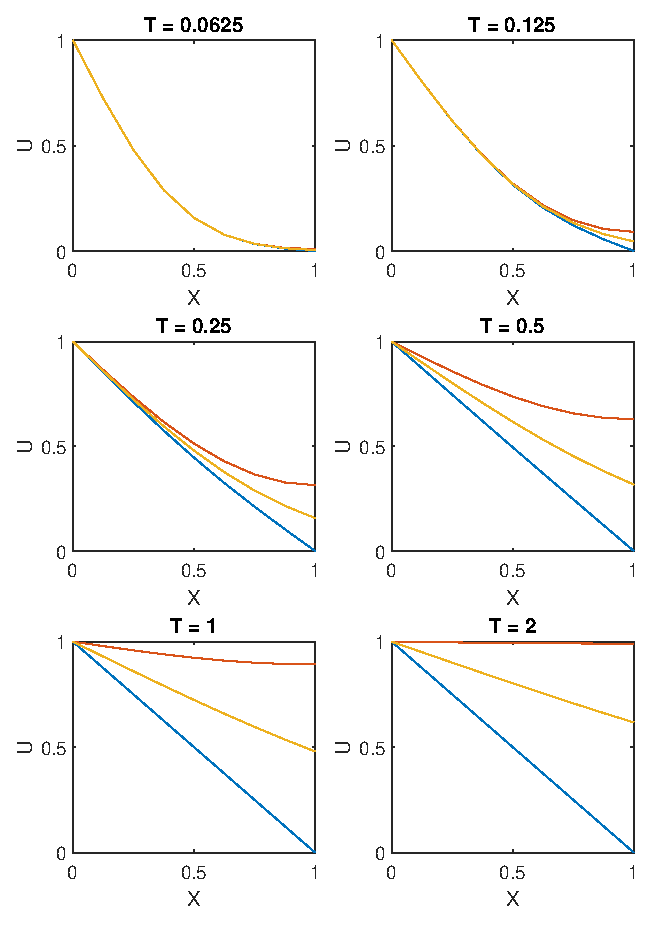
\includegraphics[scale=1.3]{Q2_TempPlot.eps}\\
\caption{Plots of the solutions against X. (17) in blue, (18) in red, (10)-(11) in yellow.}
\label{figure:1}
\end{figure} 

\begin{figure}[htp!]
\centering
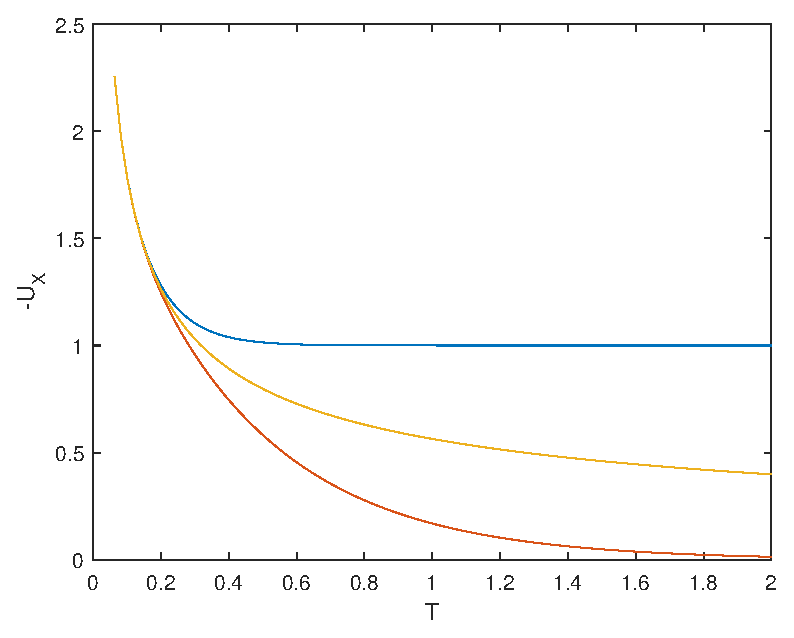
\includegraphics[scale=1]{Q2_HeatFluxPlot.eps}\\
\caption{Non-dimensionalised heat flux $-U_X$ against $T$ at $X=0$}
\label{figure:2}
\end{figure} 

\begin{figure}[htp!]
\centering
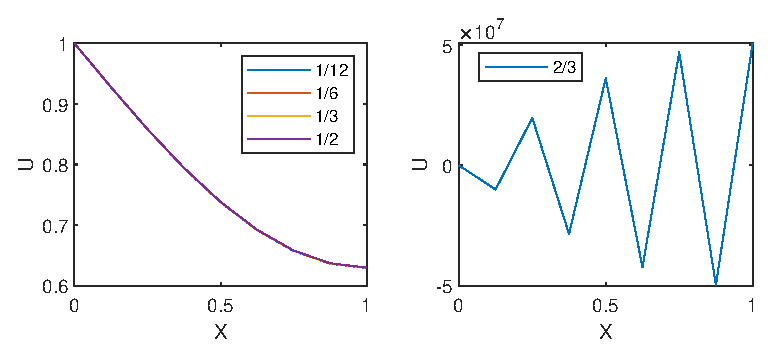
\includegraphics[width = 16cm, height = 8cm]{Q3_8_05.eps}\\
\caption{Plots of the numerical solutions with $N=8$ and $T=0.5$}
\label{figure:3}
\end{figure} 

\begin{figure}[htp!]
\centering
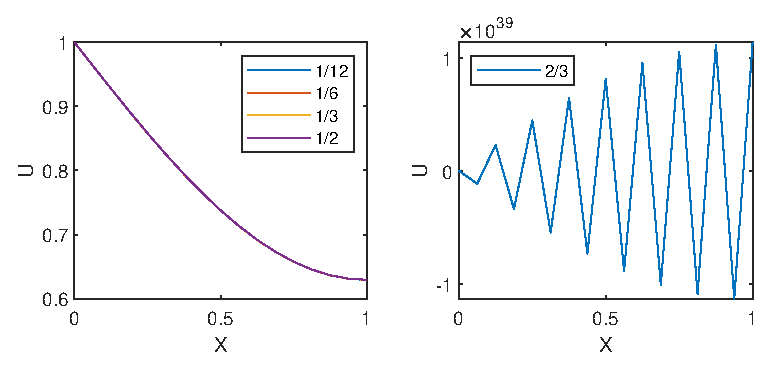
\includegraphics[width = 16cm, height = 8cm]{Q3_16_05.eps}\\
\caption{Plots of the numerical solutions with $N=16$ and $T=0.5$}
\label{figure:4}
\end{figure} 

\begin{figure}[htp!]
\centering
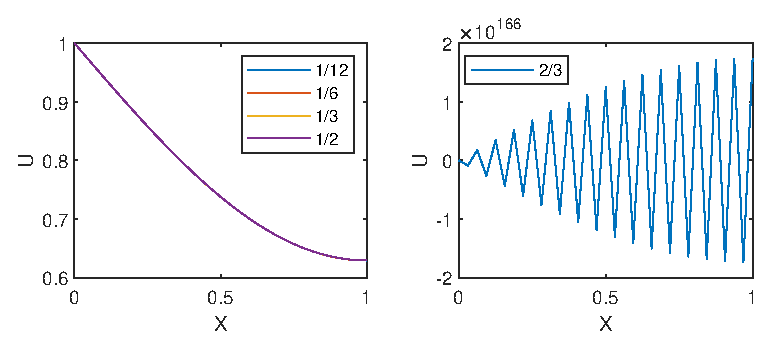
\includegraphics[width = 16cm, height = 8cm]{Q3_32_05.eps}\\
\caption{Plots of the numerical solutions with $N=32$ and $T=0.5$}
\label{figure:5}
\end{figure} 

\begin{figure}[htp!]
\centering
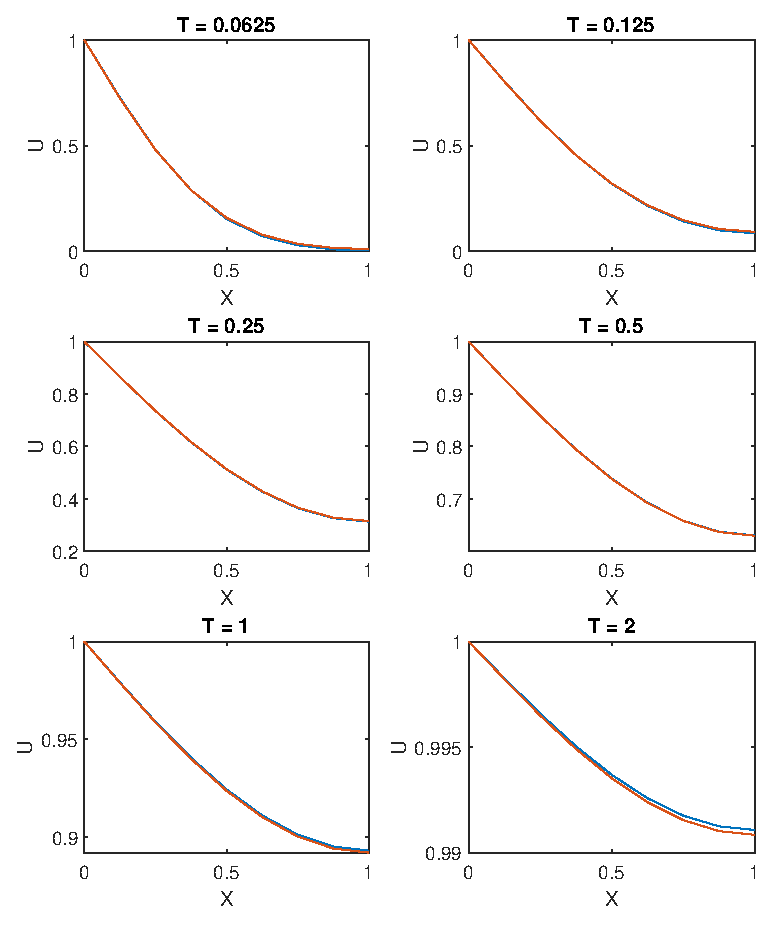
\includegraphics[scale =1.3]{Q3_ii.eps}\\
\caption{Plots of the analytic (red) and numerical (blue) solutions. }
\label{figure:6}
\end{figure} 

\pagebreak 

\textbf{Tables}

\begin{table}[htp!]
\caption{Solutions (17), (18) and (10)-(11) at $T = 0.25$}
\centering
\begin{tabular}{cccc}
\\
$X$ & (17) & (18) & (10)-(11) \\ [0.5ex]
0.0000 & 1.0000 & 1.0000 & 1.0000 \\ 
0.1250 & 0.8543 & 0.8650 & 0.8597 \\ 
0.2500 & 0.7118 & 0.7355 & 0.7237 \\ 
0.3750 & 0.5751 & 0.6167 & 0.5959 \\ 
0.5000 & 0.4460 & 0.5130 & 0.4795 \\ 
0.6250 & 0.3251 & 0.4284 & 0.3768 \\ 
0.7500 & 0.2118 & 0.3658 & 0.2888 \\ 
0.8750 & 0.1044 & 0.3275 & 0.2159 \\ 
1.0000 & -0.0000 & 0.3146 & 0.1573 \\ 
\end{tabular}
\label{table:1}
\end{table}

\begin{table}[htp!]
\caption{Analytic and numerical solutions, and the error, at $T=0.125$ with $N=8$, $C=1/2$ }
\centering
\begin{tabular}{cccc}
\\
$X$ & Analytic & Numerical & Error \\ [0.5ex]
0.0000 & 1.0000 & 1.0000 & 0.0000e+00 \\ 
0.1250 & 0.8027 & 0.8036 & 9.0710e-04 \\ 
0.2500 & 0.6175 & 0.6183 & 7.8311e-04 \\ 
0.3750 & 0.4544 & 0.4550 & 6.1037e-04 \\ 
0.5000 & 0.3200 & 0.3187 & 1.3147e-03 \\ 
0.6250 & 0.2173 & 0.2143 & 2.9645e-03 \\ 
0.7500 & 0.1460 & 0.1410 & 5.0120e-03 \\ 
0.8750 & 0.1046 & 0.0981 & 6.4838e-03 \\ 
1.0000 & 0.0910 & 0.0842 & 6.8025e-03 \\ 
\end{tabular}
\label{table:2}
\end{table}

\begin{table}[htp!]
\caption{Analytic and numerical solutions, and the error, at $T=0.25$ with $N=8$, $C=1/2$ }
\centering
\begin{tabular}{cccc}
\\
$X$ & Analytic & Numerical & Error \\ [0.5ex]
0.0000 & 1.0000 & 1.0000 & 0.0000e+00 \\ 
0.1250 & 0.8650 & 0.8649 & 9.1641e-05 \\ 
0.2500 & 0.7355 & 0.7352 & 3.1871e-04 \\ 
0.3750 & 0.6167 & 0.6161 & 5.1469e-04 \\ 
0.5000 & 0.5130 & 0.5120 & 9.8984e-04 \\ 
0.6250 & 0.4284 & 0.4271 & 1.3071e-03 \\ 
0.7500 & 0.3658 & 0.3640 & 1.8169e-03 \\ 
0.8750 & 0.3275 & 0.3255 & 1.9895e-03 \\ 
1.0000 & 0.3146 & 0.3124 & 2.2014e-03 \\ 
\end{tabular}
\label{table:3}
\end{table}

\begin{table}[htp!]
\caption{Analytic and numerical solutions, and the error, at $T=0.5$ with $N=8$, $C=1/2$ }
\centering
\begin{tabular}{cccc}
\\
$X$ & Analytic & Numerical & Error \\ [0.5ex]
0.0000 & 1.0000 & 1.0000 & 0.0000e+00 \\ 
0.1250 & 0.9277 & 0.9278 & 1.1560e-04 \\ 
0.2500 & 0.8581 & 0.8583 & 1.9953e-04 \\ 
0.3750 & 0.7940 & 0.7943 & 3.2736e-04 \\ 
0.5000 & 0.7378 & 0.7382 & 3.6568e-04 \\ 
0.6250 & 0.6917 & 0.6922 & 4.8604e-04 \\ 
0.7500 & 0.6574 & 0.6579 & 4.7387e-04 \\ 
0.8750 & 0.6363 & 0.6369 & 5.7007e-04 \\ 
1.0000 & 0.6292 & 0.6297 & 5.1116e-04 \\ 
\end{tabular}
\label{table:4}
\end{table}

\begin{table}[htp!]
\caption{Analytic and numerical solutions, and the error, at $T=1.0$ with $N=8$, $C=1/2$}
\centering
\begin{tabular}{cccc}
\\
$X$ & Analytic & Numerical & Error \\ [0.5ex]
0.0000 & 1.0000 & 1.0000 & 0.0000e+00 \\ 
0.1250 & 0.9789 & 0.9791 & 2.0096e-04 \\ 
0.2500 & 0.9587 & 0.9591 & 3.8649e-04 \\ 
0.3750 & 0.9400 & 0.9406 & 5.7227e-04 \\ 
0.5000 & 0.9236 & 0.9244 & 7.1413e-04 \\ 
0.6250 & 0.9102 & 0.9111 & 8.5647e-04 \\ 
0.7500 & 0.9002 & 0.9012 & 9.3306e-04 \\ 
0.8750 & 0.8941 & 0.8951 & 1.0103e-03 \\ 
1.0000 & 0.8920 & 0.8930 & 1.0099e-03 \\ 
\end{tabular}
\label{table:5}
\end{table}

\begin{table}[htp!]
\caption{Analytic and numerical solutions, and the error, at $T=0.5$ with $N=16$, $C=1/2$ }
\centering
\begin{tabular}{cccc}
\\
$X$ & Analytic & Numerical & Error \\ [0.5ex]
0.0000 & 1.0000 & 1.0000 & 0.0000e+00 \\ 
0.0625 & 0.9637 & 0.9637 & 1.4066e-05 \\ 
0.1250 & 0.9277 & 0.9277 & 2.7132e-05 \\ 
0.1875 & 0.8924 & 0.8924 & 4.1581e-05 \\ 
\vdots & \vdots & \vdots & \vdots\\
0.8125 & 0.6452 & 0.6453 & 1.3424e-04 \\ 
0.8750 & 0.6363 & 0.6365 & 1.3320e-04 \\ 
0.9375 & 0.6310 & 0.6311 & 1.3934e-04 \\ 
1.0000 & 0.6292 & 0.6294 & 1.3567e-04 \\ 
\end{tabular}
\label{table:6}
\end{table}

\begin{table}[htp!]
\caption{Analytic and numerical solutions, and the error, at $T=0.5$ with $N=32$, $C=1/2$ }
\centering
\begin{tabular}{cccc}
\\
$X$ & Analytic & Numerical & Error \\ [0.5ex]
0.0000 & 1.0000 & 1.0000 & 0.0000e+00 \\ 
0.0313 & 0.9818 & 0.9818 & 1.7465e-06 \\ 
0.0625 & 0.9637 & 0.9637 & 3.4616e-06 \\ 
0.0938 & 0.9456 & 0.9456 & 5.2201e-06 \\ 
\vdots & \vdots & \vdots & \vdots     \\
0.9063 & 0.6332 & 0.6333 & 3.4317e-05 \\ 
0.9375 & 0.6310 & 0.6310 & 3.4247e-05 \\ 
0.9688 & 0.6297 & 0.6297 & 3.4634e-05 \\ 
1.0000 & 0.6292 & 0.6293 & 3.4404e-05 \\ 
\end{tabular}
\label{table:7}
\end{table}

\begin{table}[htp!]
\caption{Analytic and numerical solutions, and the error, at $T=0.5$ with $N=8$, $C=1/6$ }
\centering
\begin{tabular}{cccc}
\\
$X$ & Analytic & Numerical & Error \\ [0.5ex]
0.0000 & 1.0000 & 1.0000 & 0.0000e+00 \\ 
0.1250 & 0.9277 & 0.9277 & 1.0350e-07 \\ 
0.2500 & 0.8581 & 0.8581 & 2.0051e-07 \\ 
0.3750 & 0.7940 & 0.7940 & 2.8563e-07 \\ 
0.5000 & 0.7378 & 0.7378 & 3.5535e-07 \\ 
0.6250 & 0.6917 & 0.6917 & 4.0822e-07 \\ 
0.7500 & 0.6574 & 0.6574 & 4.4452e-07 \\ 
0.8750 & 0.6363 & 0.6363 & 4.6546e-07 \\ 
1.0000 & 0.6292 & 0.6292 & 4.7228e-07 \\ 
\end{tabular}
\label{table:8}
\end{table}

\begin{table}[htp!]
\caption{Analytic and numerical solutions, and the error, at $T=0.5$ with $N=8$, $C=1/12$ }
\centering
\begin{tabular}{cccc}
\\
$X$ & Analytic & Numerical & Error \\ [0.5ex]
0.0000 & 1.0000 & 1.0000 & 0.0000e+00 \\ 
0.1250 & 0.9277 & 0.9276 & 2.7354e-05 \\ 
0.2500 & 0.8581 & 0.8580 & 5.3488e-05 \\ 
0.3750 & 0.7940 & 0.7939 & 7.7285e-05 \\ 
0.5000 & 0.7378 & 0.7377 & 9.7815e-05 \\ 
0.6250 & 0.6917 & 0.6916 & 1.1437e-04 \\ 
0.7500 & 0.6574 & 0.6573 & 1.2647e-04 \\ 
0.8750 & 0.6363 & 0.6362 & 1.3383e-04 \\ 
1.0000 & 0.6292 & 0.6291 & 1.3629e-04 \\ 
\end{tabular}
\label{table:9}
\end{table}


\pagebreak

\begin{center}
\textbf{Code for Plotting Temperature Profiles, Q2}
\end{center}
\lstinputlisting[language=Matlab]{Q2_UagainstX.m}

\begin{center}
\textbf{Code for Plotting Heat Flux, Q2}
\end{center}
\lstinputlisting[language=Matlab]{Q2_UXagainstT.m}

\begin{center}
\textbf{Code for Q3}
\end{center}
\lstinputlisting[language=Matlab]{Q3.m}

\end{document}
